\begin{center}
    \textbf{\Huge{Software Design Description (SDD)}}
\end{center}

\section{Introdução}

\subsection{Propósito}
Descrever a arquitetura e o projeto detalhado do sistema, incluindo decisões de projeto, componentes, interfaces e comportamento.

\subsection{Escopo}
Definir os limites do sistema e o que está coberto por este documento.

\subsection{Definições, Acrônimos e Abreviações}
\begin{itemize}
    \item SDD -- Software Design Description
    \item UML -- Unified Modeling Language
\end{itemize}

\subsection{Referências}
\begin{itemize}
    \item Documento de Requisitos de Software (SRS)
    \item IEEE 1016
    \item ISO/IEC/IEEE 12207
\end{itemize}

\subsection{Visão Geral do Documento}
Breve descrição da organização deste documento.

\newpage

\section{Visão Geral do Sistema}

\subsection{Contexto do Sistema}
Descrever como o sistema se insere no ambiente maior (diagramas de contexto são bem-vindos).

\subsection{Objetivos de Projeto}
\begin{itemize}
    \item Desempenho
    \item Segurança
    \item Escalabilidade
\end{itemize}

\subsection{Restrições e Premissas}
\begin{itemize}
    \item Tecnológicas
    \item Operacionais
\end{itemize}

\section{Arquitetura do Sistema (High-Level Design)}

\subsection{Visão Arquitetural}
Descrição geral da arquitetura (ex: microserviços, monolito, distribuído).

\subsection{Diagrama de Componentes}

\begin{figure}[htbp]
    \centering
    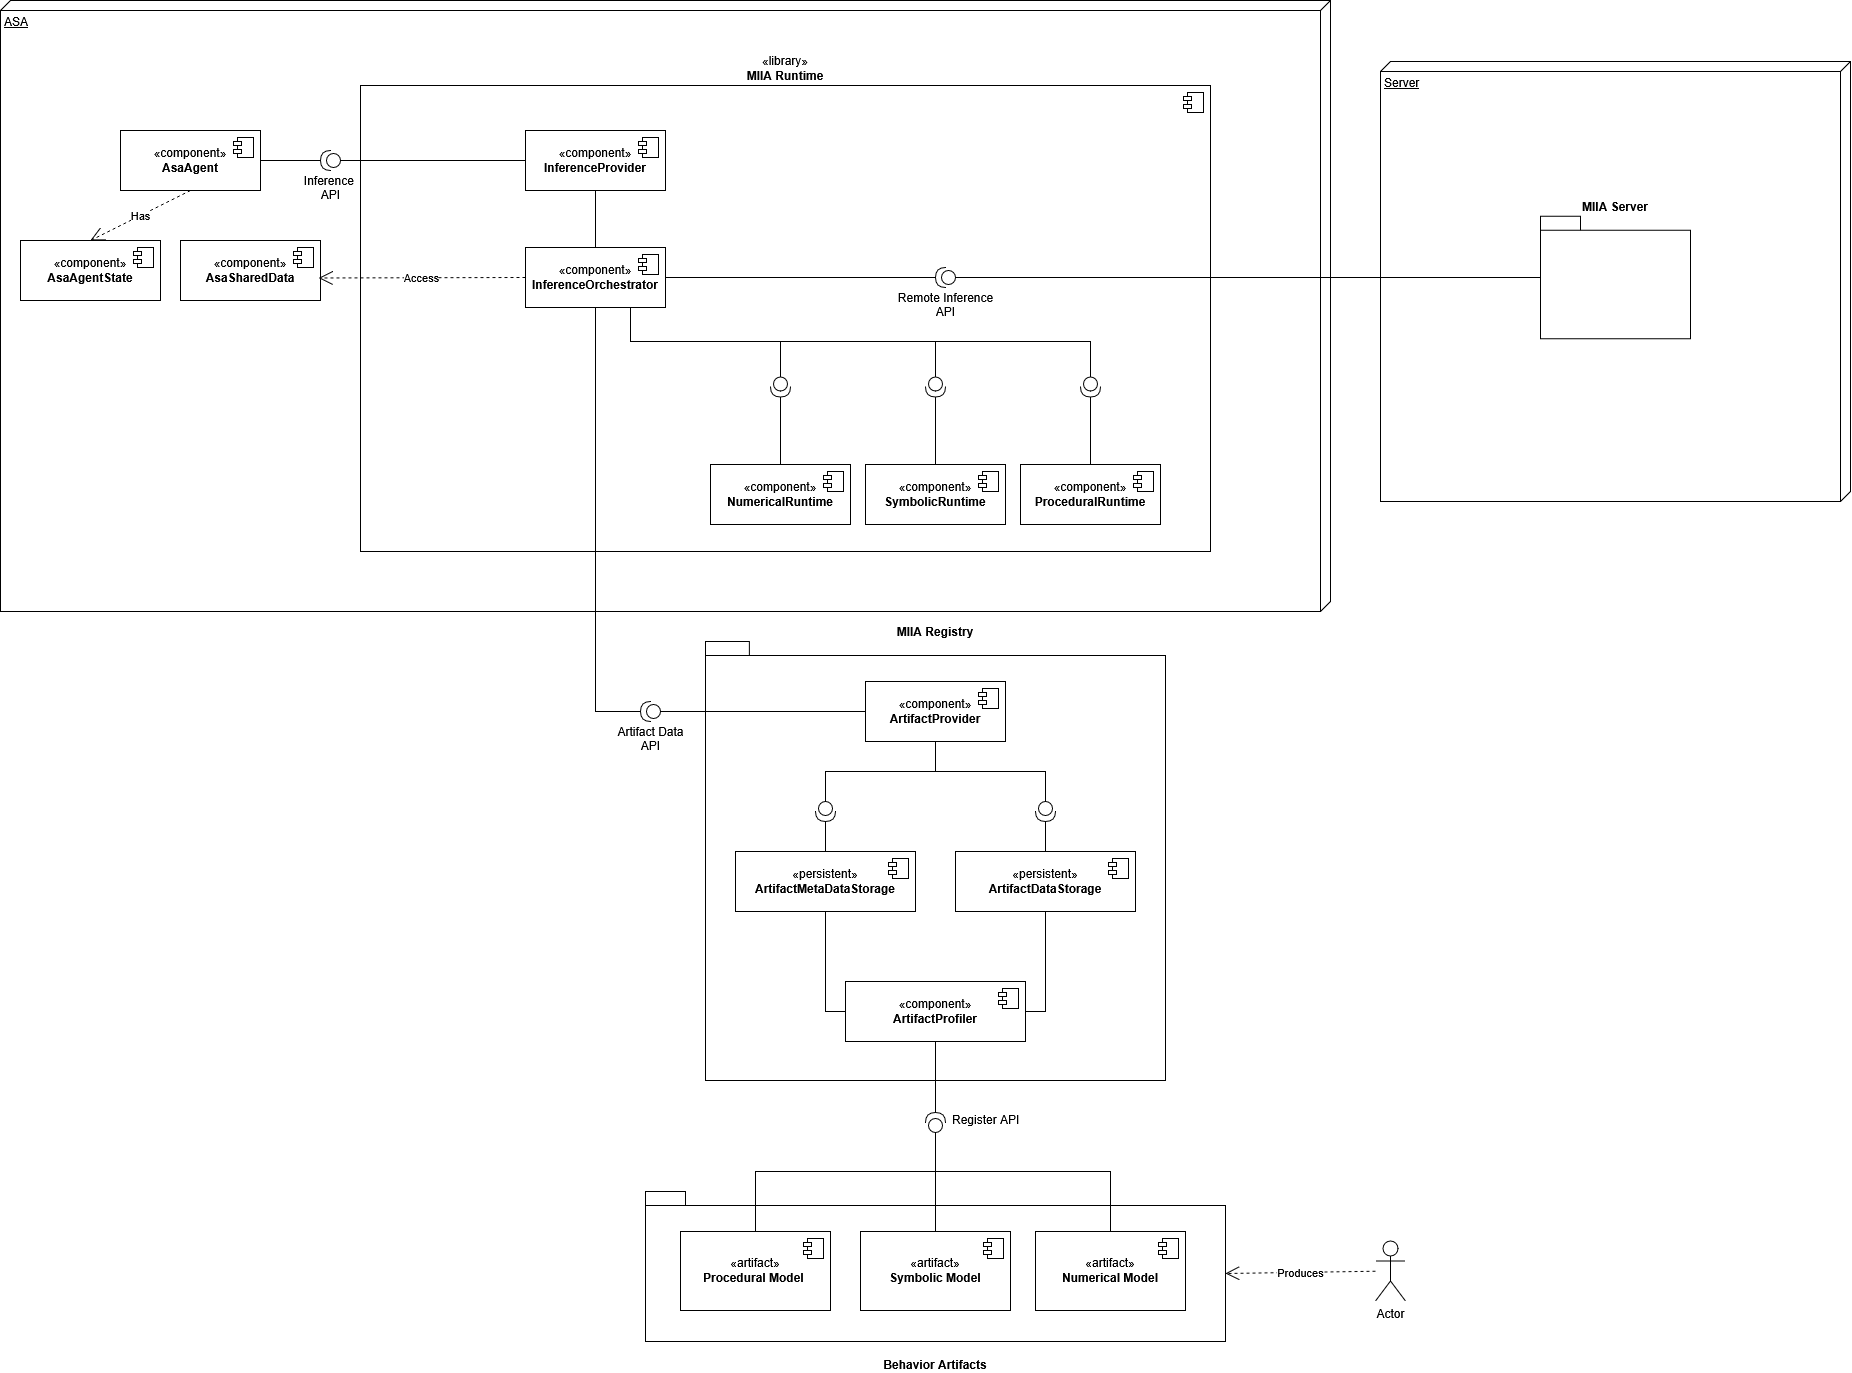
\includegraphics[width=0.8\textwidth]{./content/img/high-level-design-components.png}
    \caption{Arquitetura do MIIA - Mecanismos de Interoperabilidade de Inteligência Artificial.}
    \label{fig:olston-tfserving}
\end{figure}

\begin{center}
    % \includegraphics{component_diagram.png}
\end{center}

\subsection{Descrição dos Componentes}
\begin{itemize}
    \item Nome do componente
    \begin{itemize}
        \item Responsabilidade
        \item Interfaces fornecidas
        \item Dependências
    \end{itemize}
\end{itemize}

\subsection{Visão de Implantação (Deployment)}
Descrição de como os componentes são distribuídos em hardware/infraestrutura.

\subsection{Fluxos Principais}
Descrever fluxos importantes do sistema (pode usar diagramas de sequência).

\section{Projeto Detalhado (Low-Level Design)}

\subsection{Estrutura Interna dos Componentes}
\begin{itemize}
    \item Classes principais
    \item Módulos
\end{itemize}

\subsection{Diagramas de Classe}
% Inserir diagramas UML de classes

\subsection{Diagramas de Sequência}
% Fluxos detalhados

\subsection{Máquinas de Estado}
% Para componentes com comportamento complexo

\subsection{Algoritmos Relevantes}
Descrição de lógica crítica (sem virar código ainda).

\section{Interfaces}

\subsection{Interfaces Externas}
APIs, protocolos, integração com outros sistemas.

\subsection{Interfaces Internas}
Comunicação entre componentes.

\section{Dados}

\subsection{Modelo de Dados}
Diagramas ER ou estruturas principais.

\subsection{Dicionário de Dados}
Definição dos principais dados manipulados.

\section{Requisitos Não Funcionais}

\subsection{Desempenho}
\subsection{Segurança}
\subsection{Confiabilidade}
\subsection{Escalabilidade}

\section{Rastreabilidade}

\subsection{Mapeamento Requisito $\rightarrow$ Design}
Tabela ligando requisitos do SRS aos componentes/decisões de projeto.

\section{Decisões de Projeto e Racional}

Descrever decisões importantes e por que foram tomadas.

\section{Anexos}

\subsection{Diagramas Complementares}
\subsection{Detalhes Técnicos Adicionais}